
\chapter{Level1B data format and quality}


\section{Data format}

\smr\ Level0 and Level1B data are stored in tables
in a calibration database at the Dept. of Earth and Space
Sciences at Chalmers University of Technology (Chalmers) in Gothenburg.
There are several ways to access the data but the recommendation is to access
data through a hierarcical REST API. An online API documentation can be found at:
\url{http://odin.rss.chalmers.se/apidocs/index.html#/}.
All GET calls return JSON objects, and the ones that provides Level1B
related data are the "Log" and "L1b" endpoints:

\begin{itemize}
    \item \url{/rest_api/<version>/level1/<freqmode>/<scanno>/Log/}: Get log info for a scan
    \item \url{/rest_api/<version>/level1/<freqmode>/<scanno>/L1b/}: Get level1 data for a scan
\end{itemize}

The content of the JSON objects returned by these endpoints are described in
Table~\ref{table:logdataformat} and Table~\ref{table:dataformat}.

\begin{table}
\caption{Content description of Level1 log data of a scan as returned from GET calls to
\url{/rest_api/<version>/level1/<freqmode>/<scanno>/Log/}.
Latitudes and longitudes are given as geodetic
coordinates using WGS84 reference ellipsoid.
}
\label{table:logdataformat}
\begin{longtable}{| p{.20\textwidth} | p{.70\textwidth} |}
\hline
  \textbf{Variable} & \textbf{Description} \\
  \hline
    AltEnd                & \emph{(Double)}: Tangent point altitude ([\,m\,]) for last spectrum in scan. \\ \hline
    AltStart              & \emph{(Double)}: Tangent point altitude for first spectrum in scan. \\ \hline
    DateTime              & \emph{(String)}: Mean UTC datetime (datetime(firts) + datetime(last))/2 of scan. \\ \hline
    LatEnd                & \emph{(Double)}: Latitude of tangent point for last spectrum in scan. \\ \hline
    LatStart              & \emph{(Double)}: Latitude at tangent point for first spectrum in scan. \\ \hline
    LonEnd                & \emph{(Double)}: Longitude of tangent point for last spectrum in scan. \\ \hline
    LonStart              & \emph{(Double)}: Longitude at tangent point for first spectrum in scan. \\ \hline
    FreqMode              & \emph{(Integer)}: Deployed frequency mode. \\ \hline
    MJDEnd                & \emph{(Double)}: Modified julian date for last spectrum in scan. \\ \hline
    MJDStart              & \emph{(Double)}: Modified julian date for first spectrum in scan. \\ \hline
    NumSpec               & \emph{(Integer)}: Number of atmospheric spectra in scan. \\ \hline
    Quality               & \emph{(Integer)}: Quality estimate of the scan (see Table~\ref{table:quality}). \\ \hline
    ScanID                & \emph{(Integer)}: Satellite time word identifier of scan.\\ \hline
    SunZD                 & \emph{(Double)}: Mean solar zenith angle  (SunZD(first) + SunZD(last))/2 for scan.\\ \hline
    URLS                  & URLs to more detailed information of scan. 
                            \begin{itemize}
                             \item URL-spectra: link to scan Leve1B-data (see Table~\ref{table:dataformat})
                             \item URL-ptz: link to scan PTZ-data (see Table~\ref{table:ptzdataformat})
                             \item URL-apriori-\textit{specices} link to available scan apriori data 
                              (see Table~\ref{table:aprioridataformat}),
                              where \textit{species} can be any of: 'BrO', 'Cl2O2', 'CO', 'HCl', 'HO2', 'NO2',
                              'OCS', 'C2H2', 'ClO', 'H2CO', 'HCN', 'HOBr', 'NO', 'OH', 'C2H6', 'ClONO2', 'H2O2',
                              'HCOOH', 'HOCl', 'O2', 'SF6', 'CH3Cl', 'ClOOCl', 'H2O', 'HF', 'N2', 'O3', 'SO2',
                              'CH3CN', 'CO2', 'H2S', 'HI', 'N2O', 'OBrO', 'CH4', 'COF2', 'HBr', 'HNO3', 'NH3', 'OClO'
                            \end{itemize}
\\ \hline
                                
\hline
\end{longtable}
\end{table}
\addtocounter{table}{-1}
  

\clearpage
\newpage

\begin{table}
\caption{ Content description of \smr\ Level1B data of a scan as returned from GET calls to
(\url{/rest_api/<version>/level1/<freqmode>/<scanno>/L1b/}).
}
\label{table:dataformat}
\end{table}
\addtocounter{table}{-1}
\begin{longtable}{| p{.20\textwidth} | p{.70\textwidth} |} 
\hline
  \textbf{Variable} & \textbf{Description} \\
  \hline
     Version         & \emph{(Array of integers)}: Calibration version. \\ \hline
%     Level           & \\ \hline
     Quality         & \emph{(Array of integers)}: Quality indicator of scan/spectrum (see Table~\ref{table:quality}). \\ \hline
     STW             & \emph{(Array of integers)}: Satellite time word.\\ \hline
     MJD             & \emph{(Array of doubles)}: Modified julian date of observation. \\ \hline
     Orbit           & \emph{(Array of doubles)}: Number of orbit plus fraction. \\ \hline
%     LST             & Local sidereal time [s] of observation \\ \hline
%     Source          & \\ \hline
%     Discipline      & \\ \hline
%     Topic           & \\ \hline
     Spectrum        & \emph{(2-D Array of doubles)}: Frequency sorted and intensity calibrated spectra
                       in Rayleigh Jeans temperature in Kelvin.\\ \hline
     TrecSpectrum    & \emph{(Array of doubles)}: Frequency sorted receiver noise temperature spectrum
                       determined and used in calibration of this scan. \\ \hline
%     ObsMode         & \\ \hline
%     Type            & Type of spectrum (3=Trec, 8=atmospheric,9=SSB)\\ \hline
     Frontend        & \emph{(Array of integers)}: The frontend used for this observation: 1\,=\,555, 2\,=\,495, 
                       3\,=\,572, 4\,=\,549, and 5\,=\,119.\\ \hline
     Backend         & \emph{(Array of integers)}: The backend used for this observation: 1\,=\,AC1 and 2\,=\,AC2\\ \hline
%     SkyBeamHit      & The 16 bits of this word indicate possible hits of major
%                       sources of submillimetre emission by one of the skybeams or the
%                       main beam. E.g to test if the main beam was pointing at the Moon
%                       when a spectrum was taken during a limb scan measurement in aeronomy
%                       mode:
%                       MOONMB:  0x0200\\ \hline
     RA2000          & \emph{(Array of doubles)}: The right ascension (J2000) of the direction of pointing in degrees. \\ \hline
     Dec2000         & \emph{(Array of doubles)}: The declination (J2000) of the direction of pointing in degrees. \\ \hline
%     VSource         & \\ \hline
     Longitude       & \emph{(Array of doubles)}: Geodetic latitude of the tangent point.\\ \hline
     Latitude        & \emph{(Array of doubles)}: Geodetic latitude of the tangent point.\\ \hline
     Altitude        & \emph{(Array of doubles)}: Tangent point altitude [m].\\ \hline
%     Qtarget         & The reference attitude given as a quaternion (4-vector).\\ \hline
%     Qachieved       & The achieved attitude given as a quaternion (4-vector).\\ \hline
%     Qerror          & The attitude error in degrees, describing the pointing uncertainty
%                       around the 3 principle axes of the satellite. \\ \hline
     GPSpos          & \emph{(2-D Array of doubles)}: The geocentric position $X$,$Y$,$Z$ in meter of the satellite.\\ \hline
     GPSvel          & \emph{(2-D Array of doubles)}: The geocentric velocity $\dot X$, $\dot Y$, $\dot Z$ in meter per 
                         second of the satellite.\\ \hline
     SunPos          & \emph{(2-D Array of doubles)}: The geocentric position of the Sun in meter.\\ \hline
     MoonPos         & \emph{(2-D Array of doubles)}: The geocentric position of the Moon in meter.\\ \hline
     SunZD           & \emph{(Array of doubles)}: The solar zenith angle in degrees. \\ \hline
     Vgeo            & \emph{(Array of doubles)}: The velocity of the satellite with respect to the Earth in meter per second.\\ \hline
%     Vlsr            & \\ \hline
     Tcal            & \emph{(Array of doubles)}: The temperature in Kelvin of the calibration load.\\ \hline
     Trec            & \emph{(Array of doubles)}: The mean value of the receiver nosie temperature 
                       in Kelvin used during the intensity calibration.\\ \hline
     SBpath          & \emph{(Array of doubles)}: The path length in meter of the SSB diplexer. \\ \hline
%     LOFreq          & Local oscillator frequency in Hz in the rest frame of the satellite.\\ \hline
%     SkyFreq         & The frequency in Hz of the centre channel in the rest frame of the
%                         satellite, i.e not Doppler corrected.\\ \hline
%     RestFreq        & The frequency in Hz of the centre channel in the rest frame of the
%                         observed object, i.e Doppler corrected.\\ \hline
%     MaxSuppression  & The sideband frequency in Hz corresponding to the frequency of
%                        maximum suppression in the rest frame of the satellite,
%                        i.e not Doppler corrected.\\ \hline
     AttitudeVersion & \emph{(Array of integers)}: The version number of the attitude reconstruction software (SODA) 
                         used at SSC during production of attitiude files.\\  \hline
     FreqRes         & \emph{(Array of doubles)}: The spacing in Hz between neighbouring channels for this spectrum. \\ \hline
     FreqCal         & \emph{(2-D Array of doubles)}:  These are the four local oscillator frequencies of the SSB modules.\\ \hline
%     IntMode         & \\ \hline
     IntTime         & \emph{(Array of doubles)}: The integration time in seconds, i.e. the duration of this observation.\\ \hline
     EffTime         & \emph{(Array of doubles)}: The effective integration time in seconds, i.e. you will get the
                         noise level in this spectrum by using this time and the receiver noise 
                         temperature from above and the usual radiometer formula:
                        \begin{verbatim}dT = Trec/sqrt(df * EffTime)\end{verbatim}
                         where {\tt df} is the bandwidth (FreqRes) of the spectrometer.\\ \hline
     Channels        & \emph{(Array of integers)}: The number of channels in this spectrum.\\ \hline
     FreqMode        & \emph{(Array of integers)}: Frequency mode applied.\\ \hline
     TSpill          & \emph{(Array of doubles)}: Estimated Tspill in Kelvin. \\ \hline
     ScanID          & \emph{(Array of integers)}: satellite time word scan identifier.\\ \hline
     Apodization     & \emph{(Array of integers)}: The "channel response" filtering technique applied. 1\,=\,Hanning smoothing \\ \hline 
     Frequency       & This information can be used to create frequencys grid for the spectra,
                       and consists of four fields: \\
                     & \textbf{LOFreq}: \emph{(Array of doubles)}: Local oscillator frequency in Hz in the rest frame of the
                       observed object, i.e Doppler corrected. \\
                     & \textbf{AppliedDopplerCorr}: \emph{(Array of doubles)} The applied Doppler correction in Hz.\\
                     & \textbf{IFreqGrid}: \emph{(Array of doubles)}: The frequency grid can be obtained by
                       \begin{verbatim}frequency = LOFreq + IFreqGrid\end{verbatim}.   \\
                     & \textbf{SubBandIndex}: \emph{(2-D Array of integers)}: The SubBandIndex 
                       can be used to identify from which sub-band a given channel belongs to.
                       An example SubBandIndex array is [[ -1, -1, 420, 509, 111, 1, 310, 200],
                       [-1, -1, 508, 618, 199, 110, 419, 309]].
                       The first and second row indicate the start and end positions, respectively,
                       of the eight sub-bands in the frequency sorted spectrum.
                       The first and second index in these rows corresponds to SubBand 1 and 2, and so
                       on. E.g sub-band 3 data can be found between index 420 to 508.
                       -1 indicates that data from this band is not used. \\
                     & \textbf{ChannelsID}: \emph{(Array of integers)}: Channel identifier describes the location
                       of the sorted channels in the original unsorted spectra. \\ \hline 
     ZeroLagVar      & \emph{(2-D Array of doubles)}: Zerolag variation of the surrounding reference measurements for all sub-bands.
                       \begin{verbatim}ZeroLagVar = abs(diff(ZeroLag))/mean(ZeroLag)\end{verbatim} \([\%]\)
                        ZeroLag is the measured coefficient of the first channel of the auto-correlator,
                        and is proportional to the total power of the band. \\ \hline
\hline
\end{longtable}


\section{Quality flags}

The Quality variable of an \smr\ Level1B structure is a scalar value.
The value is determined from a quality control
of both scan variables and the individual spectrum.
Each test performed (see Table~\ref{table:quality}) is related to a unique scalar value
and the Quality variable is the sum of the values of tests 
that were not passed.  
Thus, a spectrum with a Quality value of 0 is most reliable.

The most common situation is that most spectra in a given scan has 
a Quality value of 0, and a few spectra has a higher Quality value.
In particular, the first and last spectrum of a scan tend to be more
unreliable (Quality=0x0080).  
Many scan also contain one spectrum with a Quality=0x0100
since it is common that integration times changes during a scan,
i.e. the spectra of the upper part of the scan has a greater integration 
time than spectra in the lower part of the scan.
A spectrum with Quality 0x0080 or 0x0100 does not necessarily need
to be corrupt, but the probability that it is corrupt is high.  
If the spectrum also failed to pass other tests it is corrupt. 

The radiometric noise of the spectra of a scan is estimated as decribed  
in Sect.~\ref{sec:radper} (and reported as an effective integration time (EffTime)).
This estimate does not contain the broadband noise (due to gain variation). 
The scan data contains the variable ZeroLagVar which can be seen as an estimate
of the broadband gain variation (ZeroLagVar\(\approx \frac{\Delta g}{g}\) [\%]) 
of the two surrounding references of a target spectrum.
If the ZeroLagVar is above \(\sim\)0.25 for a given sub-band
than it is likely that data from this band has a large broadband offset.
  
%\lcomment{BR}{add description of how this variable can be used to estimate broadband 
%noise level uncertainty}
 
\begin{table}
\caption{ Description of the \smr\ Quality variable. }
\label{table:quality}
\begin{longtable}{| p{.30\textwidth} | p{.50\textwidth} | p{.10\textwidth} |}
  \hline
  \textbf{Test} & \textbf{Description} & \textbf{Value} \\
  \hline
  check of Tspill   & outside of valid range (2--16\,K) & 0x0001 \\
  \hline
  check of Trec     & outside of valid range (2000--8000\,K) & 0x0002  \\
  \hline
  check of Noise    & outside of valid range. Valid range is 0.5--6\,K & 0x0004  \\
  \hline
  check of Scanning & tangent altitude is not decreasing or increasing as expected & 0x0008 \\
  \hline
  check of nr of Spectra &  the scan consists of less than five spectra & 0x0010\\
  \hline
  check of Tb       & outside of valid range (-15 -- 280\,K) & 0x0020\\ 
  \hline
  check of Tint     & integration time is outside valid range. Valid range is
                      0.85\(\pm\)0.01\,s , 1.85\(\pm\)0.01\,s, or 3.85\(\pm\)0.01\,s & 0x0040\\
  \hline
  check of References 1 & atmospheric spectrum is not collected between two sky beam 1 references     & 0x0080\\
  \hline
  check of References 2 & surrounding references have different & 0x0100\\
                        & integration times                     & \\ 
  \hline check of Moon hit   & the moon is in the main beam          & 0x0200 \\
  \hline check of Frequency    & frequency correction for \chem{CO} mode 
  (see Appendix ~\ref{chapter:freqCorrCO})
  could not be applied, and the frequency is therefore unreliable & 0x0400 \\

\hline
\end{longtable}
\end{table}
\addtocounter{table}{-1}


%\begin{figure}[t]
%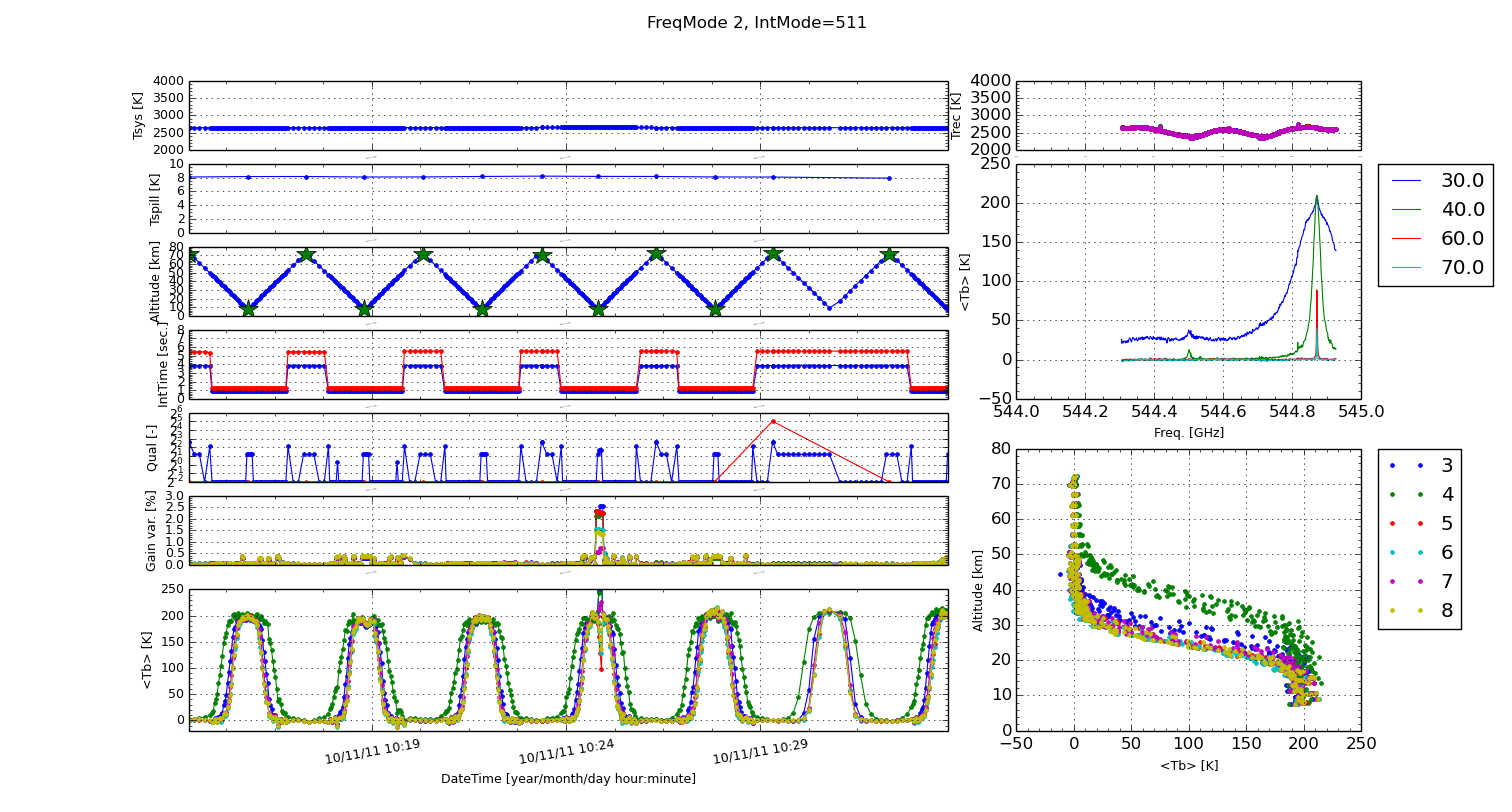
\includegraphics[width=14cm]{quality_control.png}
%\caption{Quality flag example figure\lcomment{BR}{update or remove }}
%\label{fig:quality}
%\end{figure}

    




\chapter{Summary}


Some key issues that should be considered when examining or applying \smr\
Level1B data:
\begin{itemize}

\item \smr\ can perform observations in a number of different frequency
bands, mainly within the 486\,--\,504\,GHz and 541\,--\,581\,GHz regions.
In practise, two or three frequency bands are measured simultaneously.
For a given day, several observation modes can be applied, and hence
it is rather complicated to describe the time-sharing in a 
comprehensive way.
 

\item Calibrated spectra are expressed in terms of Rayleigh--Jeans brightness temperature.

\item \smr\ spectra contain a significant amount of broadband noise, 
due to rapid gain fluctuations, in addition to radiometric noise.


\end{itemize}

